
\vspace*{-5pt}

\section{ Less powerful but still interesting GNNs}
\label{sec:theory}


\begin{figure}[!t]
 \vspace{-0.2in}
    \centering
        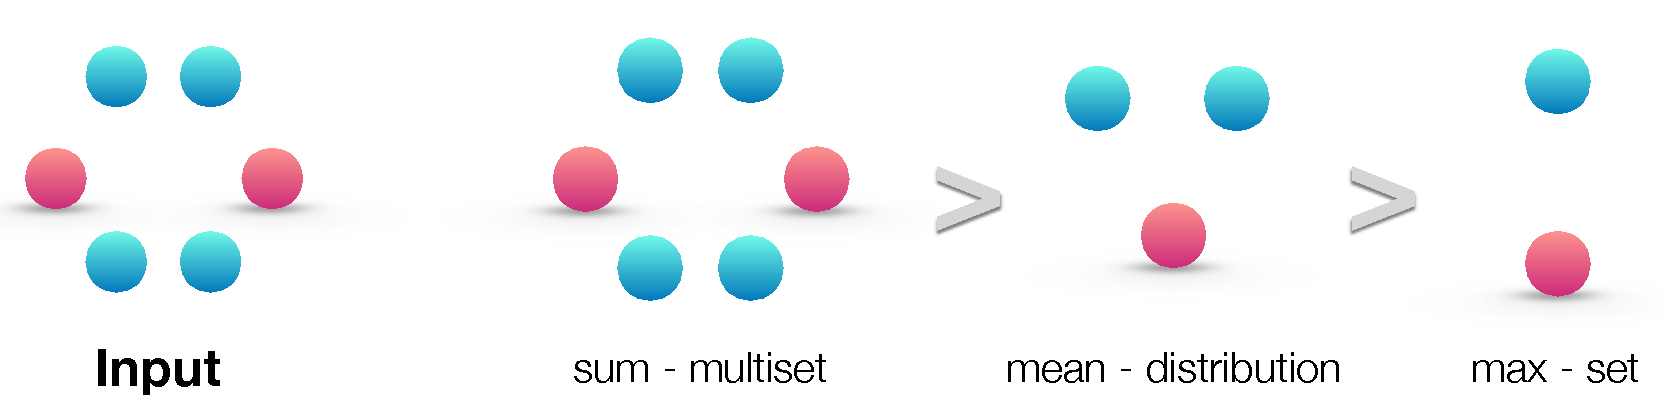
\includegraphics[width=0.85\textwidth]{rank.pdf} 
    \caption{{\bf Ranking by expressive power for sum, mean and max aggregators over a multiset}. 
    Left panel shows the input multiset, \ie, the network neighborhood to be aggregated.
    The next three panels illustrate the aspects of the multiset a given aggregator is able to capture: sum captures the full multiset, mean captures the proportion/distribution of elements of a given type, and the max aggregator ignores multiplicities (reduces the multiset to a simple set).}
\label{fig:ranking}
\end{figure}

\begin{figure}[t]
 \vspace{-0.05in}
    \centering
    \begin{subfigure}[b]{0.25\textwidth}
        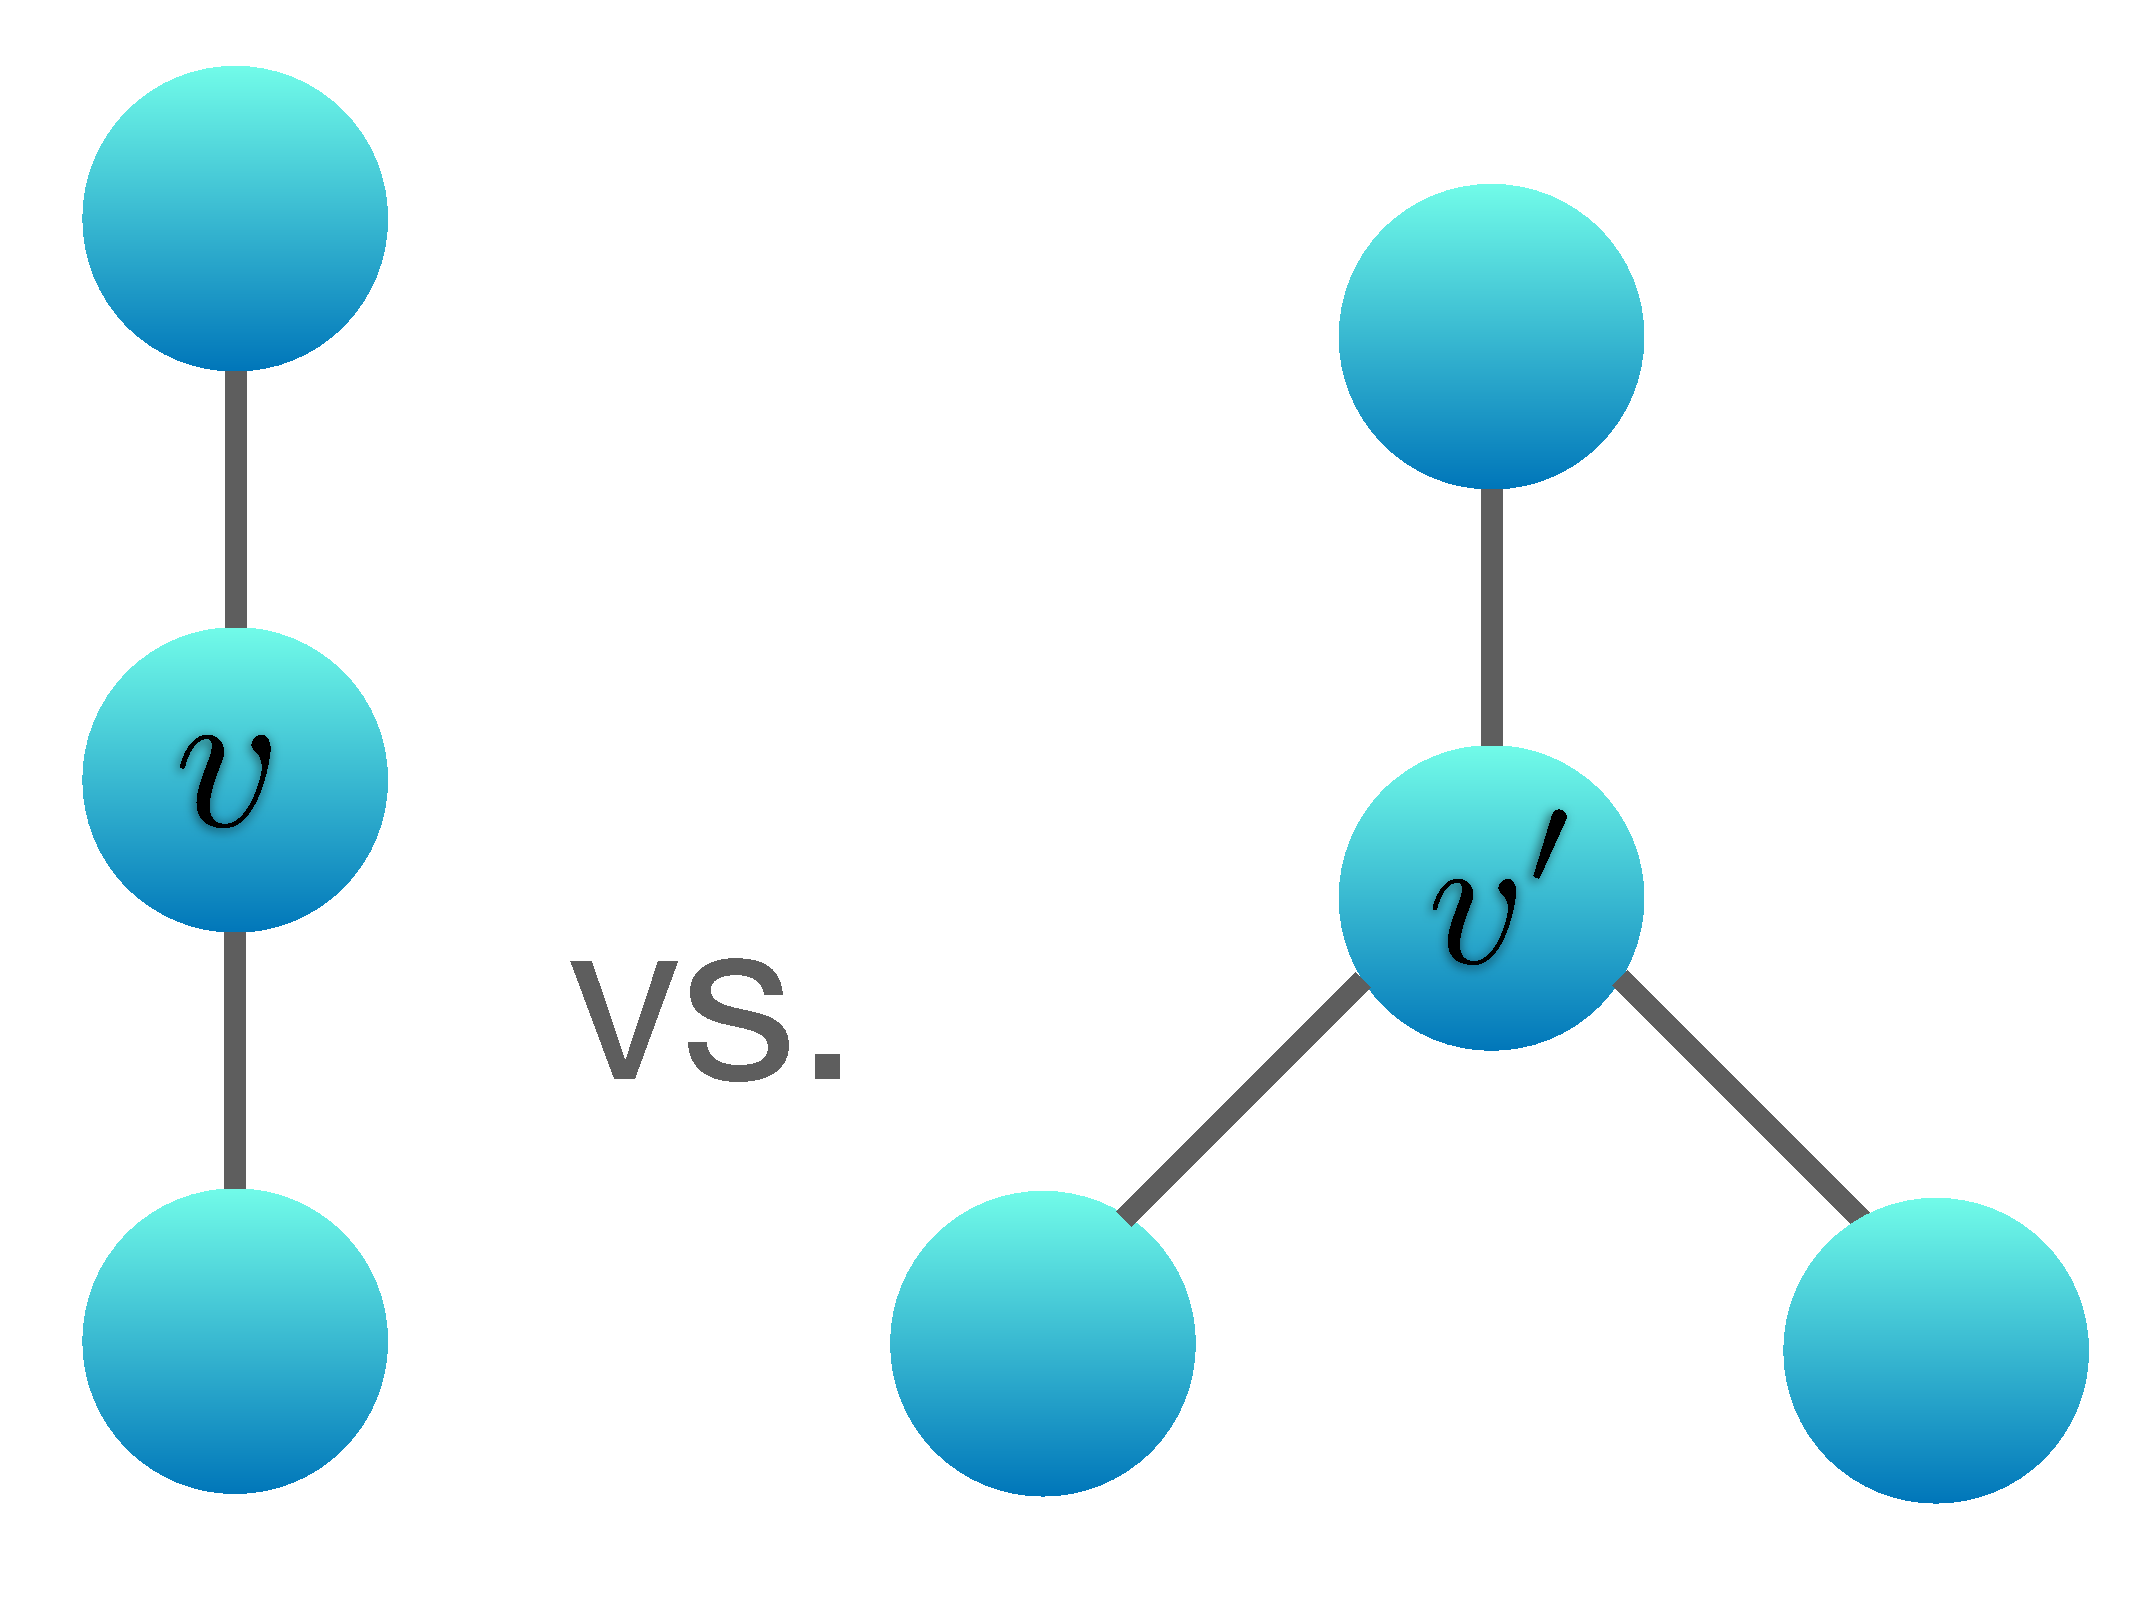
\includegraphics[width=0.95\textwidth]{graph3_center.pdf} \vspace{-0.1in}
        \caption{Mean and Max both fail}
        \label{fig:all-same}
    \end{subfigure}   \hspace{0.1\textwidth}
    \begin{subfigure}[b]{0.25\textwidth}
        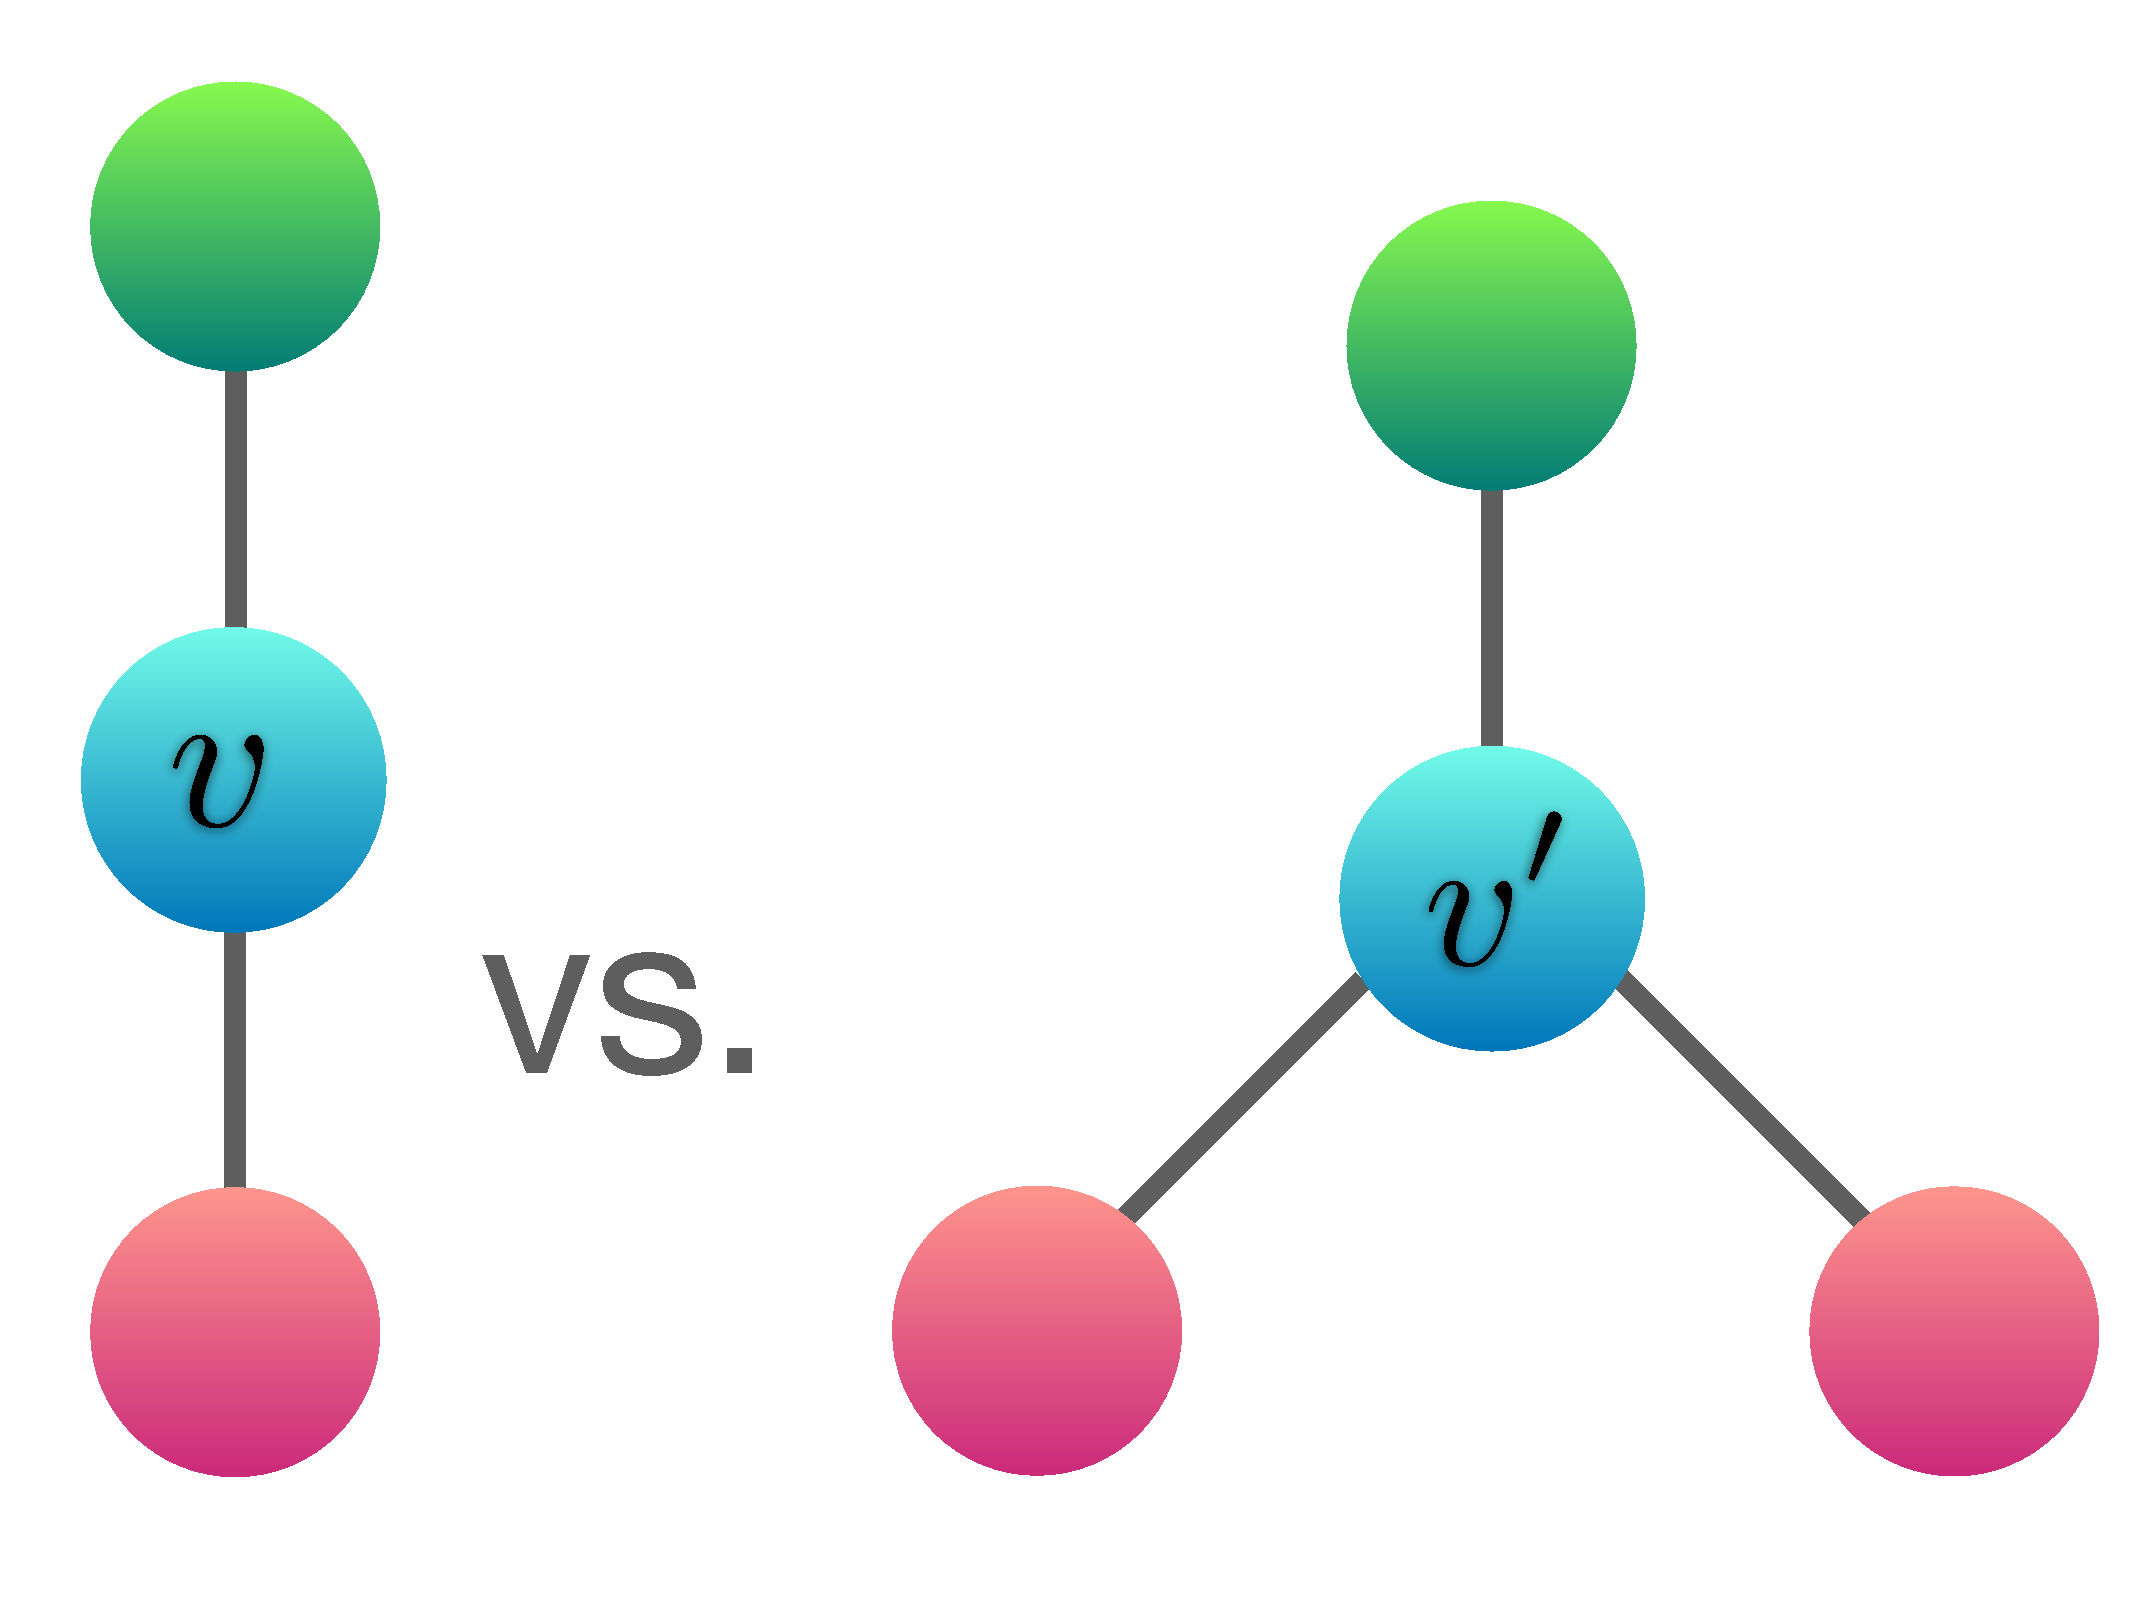
\includegraphics[width=0.95\textwidth]{graph1_center.pdf}  \vspace{-0.1in}
        \caption{Max fails}
        \label{fig:max-fail}
    \end{subfigure}   \hspace{0.1\textwidth}
    \begin{subfigure}[b]{0.25\textwidth}
        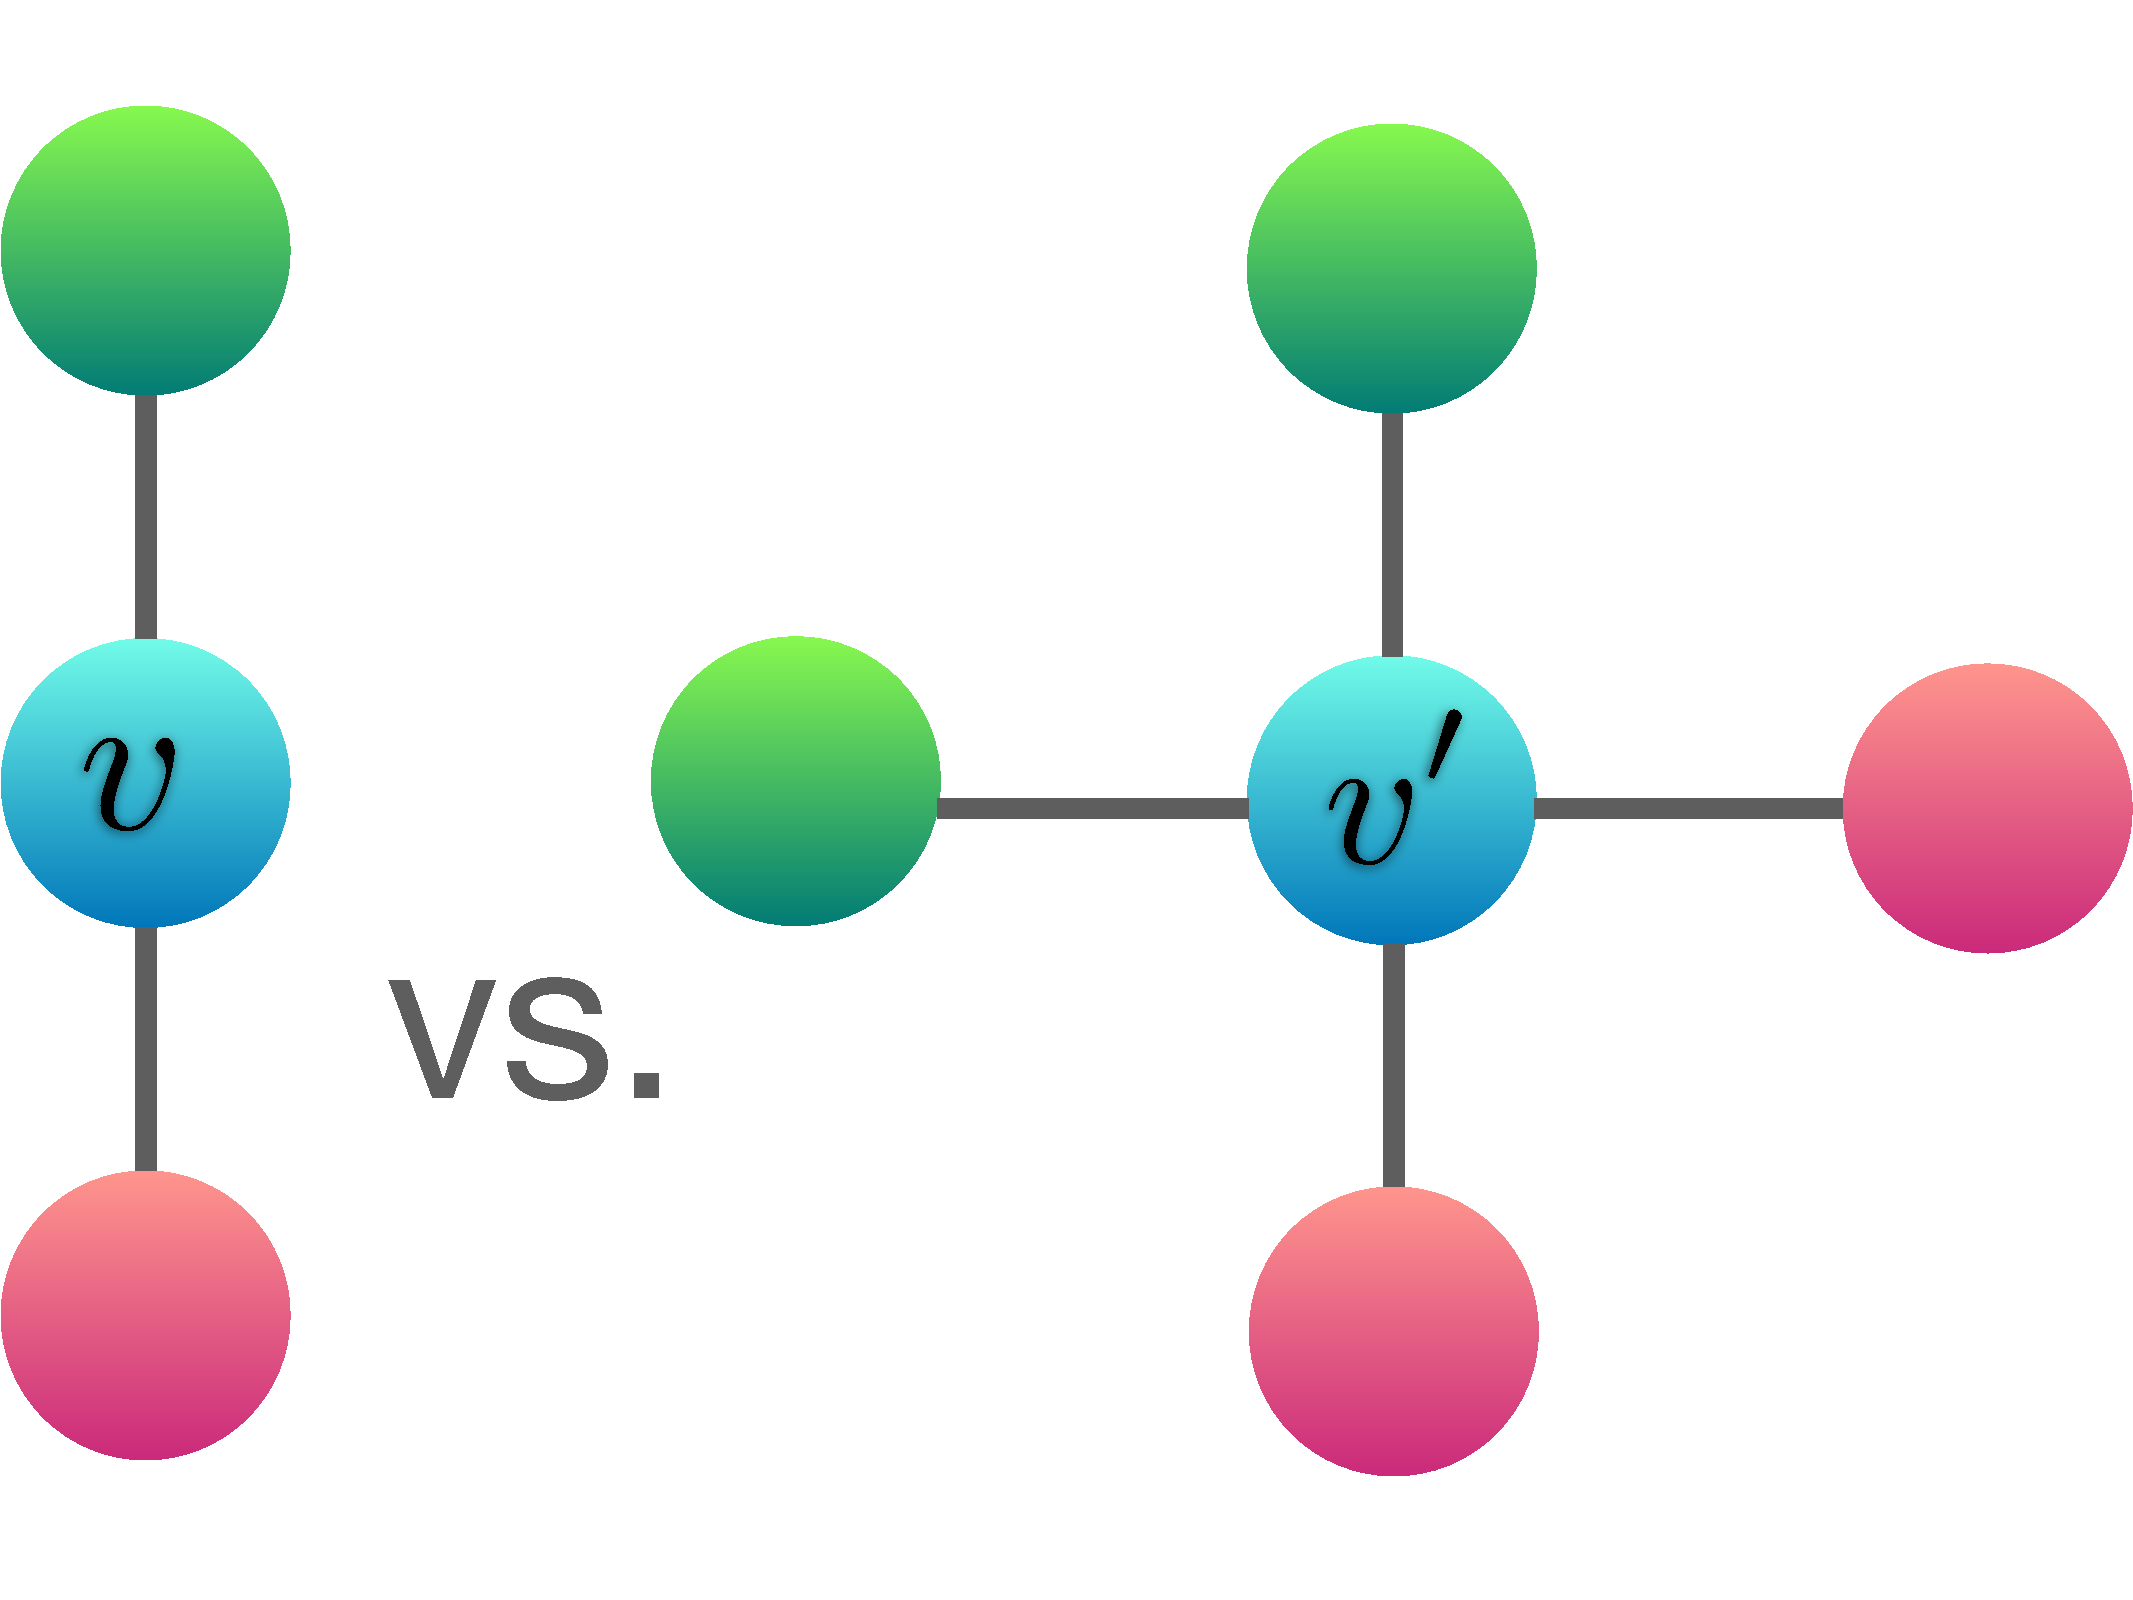
\includegraphics[width=0.95\textwidth]{graph2_center.pdf} \vspace{-0.1in}
        \caption{Mean and Max both fail}
        \label{fig:mean-fail}
    \end{subfigure}
    \caption{{\bf Examples of graph structures that mean and max aggregators fail to distinguish.} Between the two graphs, nodes $v$ and $v'$ get the same embedding even though their corresponding graph structures differ.
    Figure~\ref{fig:ranking} gives reasoning about how different aggregators ``compress'' different multisets and thus fail to distinguish them. 
    }
\label{fig:graphs-fail}
 \vspace{-0.1in}
\end{figure}

Next, we study GNNs that do not satisfy the conditions in Theorem~\ref{theorem:condition}, including GCN~\citep{kipf2016semi} and GraphSAGE~\citep{hamilton2017inductive}. We conduct ablation studies on two aspects of the aggregator in~\refeq{GIN-agg}: (1) 1-layer perceptrons instead of MLPs and (2) mean or max-pooling instead of the sum.  We will see that these GNN variants get confused by surprisingly simple graphs and are less powerful than the WL test. Nonetheless, models with mean aggregators like GCN perform well for \textit{node classification} tasks. To better understand this, we precisely characterize what different GNN variants can and cannot capture about a graph and discuss the implications for learning with graphs.

\subsection{1-layer perceptrons are not sufficient}
The function $f$ in Lemma~\ref{theorem:sum} helps map distinct multisets to unique embeddings. It can be parameterized by an MLP by the universal approximation theorem~\citep{hornik1991approximation}. Nonetheless, many existing GNNs instead use a 1-layer perceptron $\sigma \circ W$~\citep{duvenaud2015convolutional, kipf2016semi, zhang2018end}, a linear mapping followed by a non-linear activation function such as a ReLU. Such 1-layer mappings are examples of Generalized Linear Models~\citep{Neld:Wedd:1972}. Therefore, we are interested in understanding whether 1-layer perceptrons are enough for graph learning. %one can entirely substitute MLPs in the context of graph learning.
%Lemma~\ref{theorem:mlp} suggests
Lemma~\ref{theorem:mlp} suggests that there are indeed network neighborhoods (multisets) that models with 1-layer perceptrons can never distinguish.
%
\begin{lemma}
\label{theorem:mlp}
There exist finite multisets $X_1 \neq X_2$ so that for any linear mapping $W$,  $ \sum\nolimits_{x \in X_1} {\rm ReLU} \left( Wx \right) = \sum\nolimits_{x \in X_2} {\rm ReLU} \left( Wx \right). $ %\]
\end{lemma}
%
The main idea of the proof for Lemma~\ref{theorem:mlp} is that 1-layer perceptrons can behave much like linear mappings, so the GNN layers degenerate into simply summing over neighborhood features. 
\revise{Our proof builds on the fact that the bias term is lacking in the linear mapping. With the bias term and sufficiently large output dimensionality, 1-layer perceptrons might be able to distinguish different multisets. Nonetheless, unlike models using MLPs, the 1-layer perceptron (even with the bias term) is \emph{not a universal approximator} of multiset functions. Consequently, even if  GNNs with 1-layer perceptrons can embed different graphs to different locations to some degree, such embeddings may not adequately capture structural similarity, and can be difficult for simple classifiers, \eg, linear classifiers, to fit. In Section \ref{sec:experiments}, we will empirically see that GNNs with $1$-layer perceptrons, when applied to graph classification, sometimes severely underfit training data and often perform worse than GNNs with MLPs in terms of test accuracy.}



\subsection{Structures that confuse mean and max-pooling }
\label{sec:confuse}

What happens if we replace the sum in $h\left(X \right) =   \sum_{x \in X} f(x)$ with mean or max-pooling as in GCN and GraphSAGE? Mean and max-pooling aggregators are still well-defined multiset functions because they are permutation invariant. But, they are \textit{not} injective. Figure~\ref{fig:ranking} ranks the three aggregators by their representational power, and Figure~\ref{fig:graphs-fail} illustrates pairs of structures that the mean and max-pooling aggregators fail to distinguish. Here, node colors denote different node features, and we assume the GNNs aggregate neighbors first before combining them with the central node labeled as $v$ and $v'$.

In Figure~\ref{fig:all-same}, every node has the same feature $a$ and $f(a)$ is the same across all nodes (for any function $f$). When performing neighborhood aggregation, the mean or maximum over $f(a)$ remains $f(a)$ and, by induction, we always obtain the same node representation everywhere. Thus, in this case mean and max-pooling aggregators fail to capture any structural information. In contrast, the sum aggregator distinguishes the structures because $2 \cdot f(a)$ and $3 \cdot f(a)$ give different values. The same argument can be applied to any unlabeled graph. If node degrees instead of a constant value is used as node input features, in principle, mean can recover sum, but max-pooling cannot.

Fig.~\ref{fig:all-same} suggests that mean and max have trouble distinguishing graphs with nodes that have repeating features. Let $h_{{\rm color}}$ ($r$ for red, $g$ for green) denote node features transformed by $f$.
% after applying $f$. 
Fig.~\ref{fig:max-fail} shows that maximum over the neighborhood of the blue nodes $v$ and $v'$ yields $\max \left( h_{\text{g}}, h_{\text{r}} \right)$ and $\max \left( h_{\text{g}}, h_{\text{r}}, h_{\text{r}} \right)$, which collapse to the same representation (even though the corresponding graph structures are different). Thus, max-pooling fails to distinguish them. In contrast, the sum aggregator still works because $\frac{1}{2} \left( h_{\text{g}} + h_{\text{r}} \right)$ and $\frac{1}{3} \left( h_{\text{g}} + h_{\text{r}} + h_{\text{r}} \right)$ are in general not equivalent. Similarly, in Fig.~\ref{fig:mean-fail}, both mean and max fail as $\frac{1}{2} \left( h_{\text{g}} + h_{\text{r}} \right) = \frac{1}{4} \left( h_{\text{g}} +h_{\text{g}} + h_{\text{r}} + h_{\text{r}} \right)$. 

%The mean aggregator always maps two multisets, where one contains multiple copies of the other, to the same embedding. In fact, this is the only case where mean fails. Max-pooling, however, easily get confused by graphs where node features repeat.


\subsection{Mean learns distributions}
To characterize the class of multisets that the mean aggregator can distinguish, consider the example $X_1 = (S, m)$ and $X_2 = (S, k \cdot m)$, where $X_1$ and $X_2$ have the same set of distinct elements, but $X_2$ contains $k$ copies of each element of $X_1$. Any mean aggregator maps $X_1$ and $X_2$ to the same embedding, because it simply takes averages over individual element features. % because the average of $k$ instances of the same element equals one instance.
Thus, the mean captures the \textit{distribution} (proportions) of elements in a multiset, but not the \textit{exact} multiset. %Indeed, we can view it as a distributional form of the sum aggregator.
%
% \vspace{0.01in}

\begin{corollary} \label{theorem:mean}
Assume $\mathcal{X}$ is countable. There exists a function $f:\mathcal{X}\rightarrow\mathbb{R}^n$ so that for $h(X) =  \frac{1}{|X|}  \sum_{x \in X} f(x)$, $h(X_1) = h(X_2)$ if and only if multisets $X_1 $ and $X_2$ have the same distribution. That is, assuming $|X_2| \geq |X_1|$, we have $X_1 = (S, m)$ and $X_2 = (S, k \cdot m)$ for some $k \in \mathbb{N}_{\geq 1}$.
\end{corollary}
 \vspace{-0.02in}
%
The mean aggregator may perform well if, for the task, the statistical and distributional information in the graph is more important than the exact structure. Moreover, when node features are diverse and rarely repeat, the mean aggregator is as powerful as the sum aggregator. This may explain why, despite the limitations identified in Section~\ref{sec:confuse}, GNNs with mean aggregators are effective for node classification tasks, such as classifying article subjects and community detection, where node features are rich and the distribution of the neighborhood features provides a strong signal for the task.


\subsection{Max-pooling learns sets with distinct elements}
The examples in Figure~\ref{fig:graphs-fail} illustrate that max-pooling considers multiple nodes with the same feature as \textit{only one} node (\ie, treats a multiset as a set). Max-pooling captures neither the exact structure nor the distribution. However, it may be suitable for tasks where it is important to identify representative elements or the ``skeleton'', rather than to distinguish the exact structure or distribution. \citet{qi2017pointnet} empirically show that the max-pooling aggregator learns to identify the skeleton of a 3D point cloud and that it is robust to noise and outliers. For completeness, the next corollary shows that the max-pooling aggregator captures the underlying set of a multiset.
%
 \vspace{0.03in}
\begin{corollary} \label{theorem:max-pooling}
Assume $\mathcal{X}$ is countable. Then there exists a function $f:\mathcal{X}\rightarrow \mathbb{R}^{\infty}$ so that for $h(X) =  \max_{x \in X} f(x)$, $h(X_1) = h(X_2)$ if and only if $X_1 $ and $X_2$ have the same underlying set.
\end{corollary}

\subsection{Remarks on other aggregators}
\revise{There are other non-standard neighbor aggregation schemes that we do not cover, \eg, weighted average via attention~\citep{velivckovic2017graph} and LSTM pooling \citep{hamilton2017inductive, murphy2018janossy}. We emphasize that our theoretical framework is general enough to characterize the representaional power of any aggregation-based GNNs.
In the future, it would be interesting to apply our framework to analyze and understand other aggregation schemes.}


\section{Other related work}
\label{sec:related}
Despite the empirical success of GNNs, there has been relatively little work that mathematically studies their properties.  An exception to this is the work of \citet{scarselli2009computational} who shows that the perhaps earliest GNN model~\citep{scarselli2009graph} can approximate measurable functions in probability. \citet{lei2017deriving} show that their proposed architecture lies in the RKHS of graph kernels, but do not study explicitly which graphs it can distinguish. Each of these works focuses on a specific architecture and do not easily generalize to multple architectures. % and in contrast to our work here it does not generalize to multiple architectures.
In contrast, our results above provide a general framework for analyzing and characterizing the expressive power of a broad class of GNNs. 
Recently, many GNN-based architectures have been proposed, including sum aggregation and MLP encoding~\citep{battaglia2016interaction, scarselli2009graph,  duvenaud2015convolutional}, and most without theoretical derivation. In contrast to many prior GNN architectures, our Graph Isomorphism Network (GIN) is theoretically motivated, simple yet powerful.

